\section{Herangehensweise}
Für die Umsetzung des Projekts wurde agiles Projektmanagement gewählt. Im Rahmen der agilen Entwicklung wurden wöchentliche Sprints festgelegt, in denen Gruppenmitglieder den Fortschritt der jeweiligen Aufgaben präsentieren. Dies ermöglicht es, bei auftretenden Problemen gemeinsam Lösungen zu erarbeiten. Durch diese Struktur lassen sich Projektziele dynamisch anpassen, wodurch eine schnelle Reaktion auf Probleme oder Engpässe gewährleistet ist.\\

Zu Beginn wurde ein Endziel definiert, das in Abschnitt \ref{sec:vision} beschrieben ist und auf das konsequent hingearbeitet wird. Innerhalb des ersten Sprints konnte erfolgreich eine einfache Datenübertragung zwischen einem ESP32 und einem Arduino-Nano hergestellt werden.\\

In den darauf folgenden zwei Sprints wurde ein erster einfacher Prototyp des Busses entwickelt. Dieser umfasste einen Eindraht-Bus, wobei die Software zu diesem Zeitpunkt lediglich unidirektionale Kommunikation zwischen einem Sender und mehreren Empfängern unterstützte.\\

Im weiteren Verlauf des Projekts wurden Tasten sowie zusätzliche Teilnehmer auf dem Prototyp implementiert. Die Tasten dienten der Simulation verschiedener Busteilnehmer. Jedem Taster wurde ein Mikrocontroller (ATtiny oder ATmega) zugeordnet, um die Adressierung der unterschiedlichen Module zu entwickeln und zu validieren. Das gewünschte Verhalten bestand darin, dass ausschließlich der Mikrocontroller mit der entsprechenden Adresse aktiviert wird, wodurch eine LED zum Leuchten gebracht wird.\\

Anschließend wurde der Prototyp um eine weitere Busleitung erweitert und die differenzielle Datenübertragung angegangen. Hierbei sind einige Schwierigkeiten bezüglich der Hardware aufgetreten. Nach einem Neubau des Prototyps auf dem Breadboard und Reduzierung der Teilnehmer aufgrund von Platzmangel auf dem Breadboard ließ sich ein Keypad-Modul und der Hauptcontroller aufbauen (Abb. \ref{prototyp}). \\
Mit diesem Stand des Prototyps lässt sich ein 2x2 Keypad beliebig belegen und zum Beispiel eine PowerPoint-Präsentation steuern.

\begin{figure}[H]
    \centering    
    \fbox{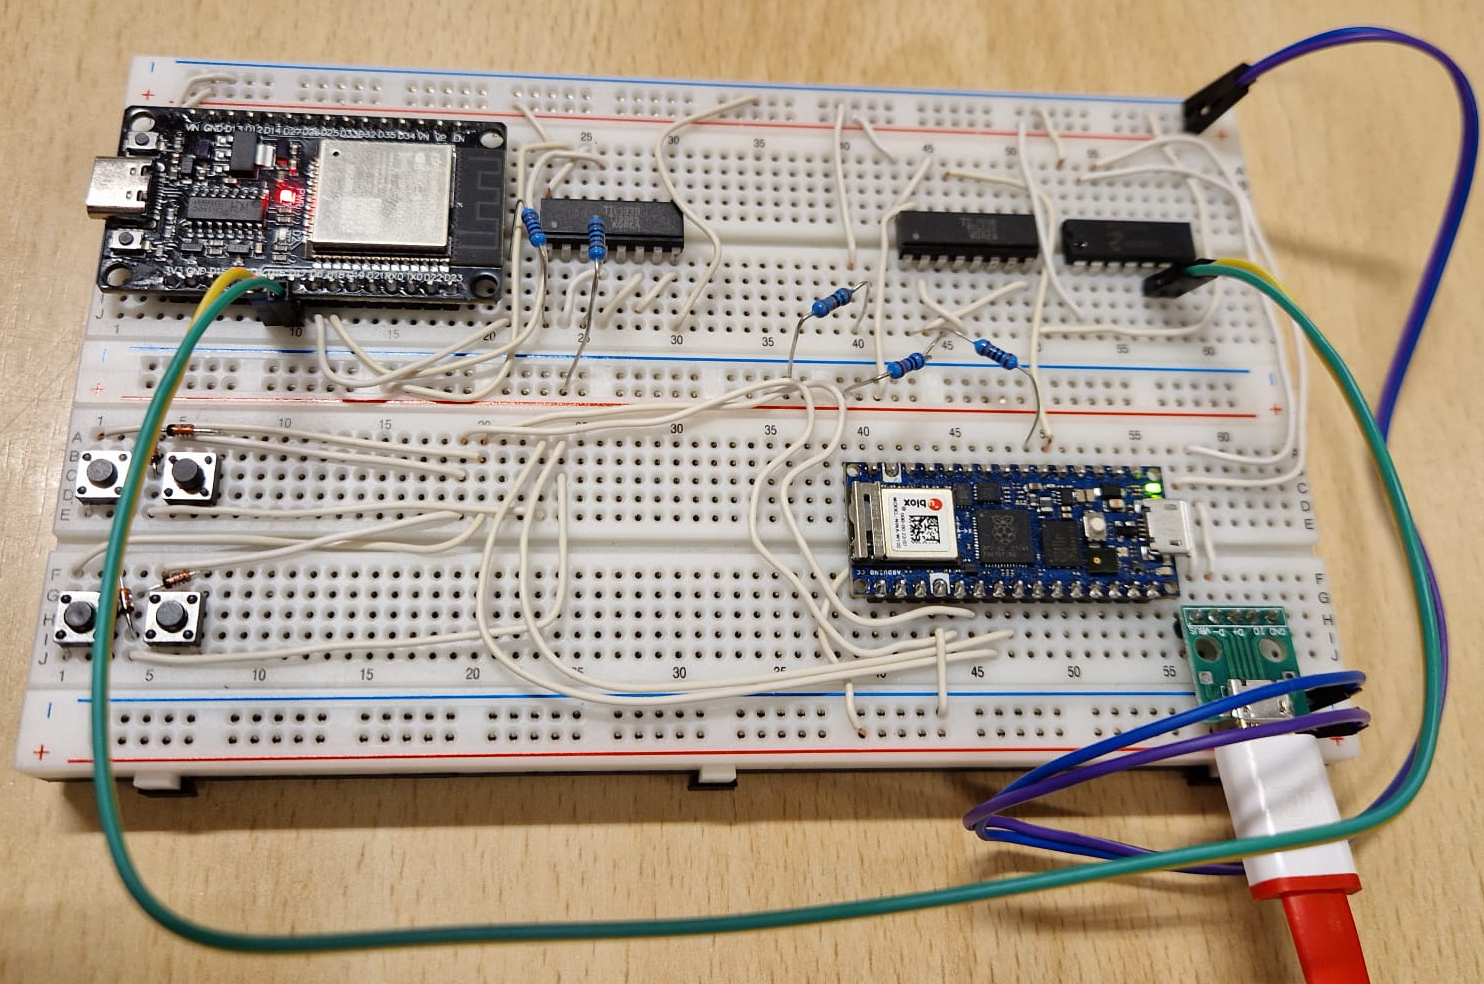
\includegraphics[width=1\textwidth]{Bilder/buPrototyp.png}}
    \caption{Aktueller Entwicklungs-Prototyp}
    \label{prototyp}
\end{figure}

\subsection{Erfolge}
\subsubsection{Synchronisation}
Zur Synchronisation des Empfängers mit dem Sender haben wir eine Funktion geschrieben, welche bei einem HIGH-Value auf dem Bus einen Zeitstempel setzt und sobald der Bus auf LOW fällt, die Übertragungsgeschwindigkeit ausrechnet. Damit wird sichergestellt, dass die übertragenen Bits richtig ausgelesen werden.

\subsubsection{Datenübertragung}
Durch die selbst geschriebene Software lassen sich in der Theorie beliebig große Datenmengen übertragen, solange die Anzahl an Datenbytes im Code festgelegt wurde. In der Praxis sind große Datenmengen vermutlich problematisch, da die Synchronisation nur zu Beginn des Frames stattfindet. Da wir in unserem Projekt nur Eingabewerte übertragen, welche 8 Byte nicht überschreiten werden, haben wir uns auf ein Maximum von 8 Byte festgelegt. Sollte sich an einem zukünftigen Entwicklungspunkt herausstellen, dass wir mehr Daten übertragen wollen, lässt sich das leicht anpassen, aber es sollte auch eventuell eine Neusynchronisation überlegt werden. 

\subsubsection{Adressvergabe und Polling loop}
Das Hauptmodul startet eine dauerhafte vordefinierte Abfrage der Adressen. Über die erste abgefragte Adresse wird einem neuen Modul eine Adresse vergeben und diese mit der Art des Moduls in Hauptmodul abgespeichert. Die erhaltenen Werte der Module gibt das Hauptmodul zusammen mit der Modul-Adresse an den PC weiter.

\subsubsection{Parallele Entwicklung}
Das parallele Entwickeln war durch das Verwenden des Versionsverwaltungs-Programms \glqq Git\grqq{} und einem zentralen Repository auf \glqq GitHub\grqq{} von Beginn an erfolgreich und hat sich durch die Länge des Projekts gezogen. Durch das Erstellen von persönlichen \glqq Branches\grqq{} konnte jeder Entwickler an seinem eigenen Fortschritt arbeiten und bei Bedarf mit dem Hauptzweig zusammenführen. In Abb. \ref{gitgraph} ist ein Ausschnitt des GitGraphen unseres Repository zu sehen.

\begin{figure}[H]
    \centering    
    \fbox{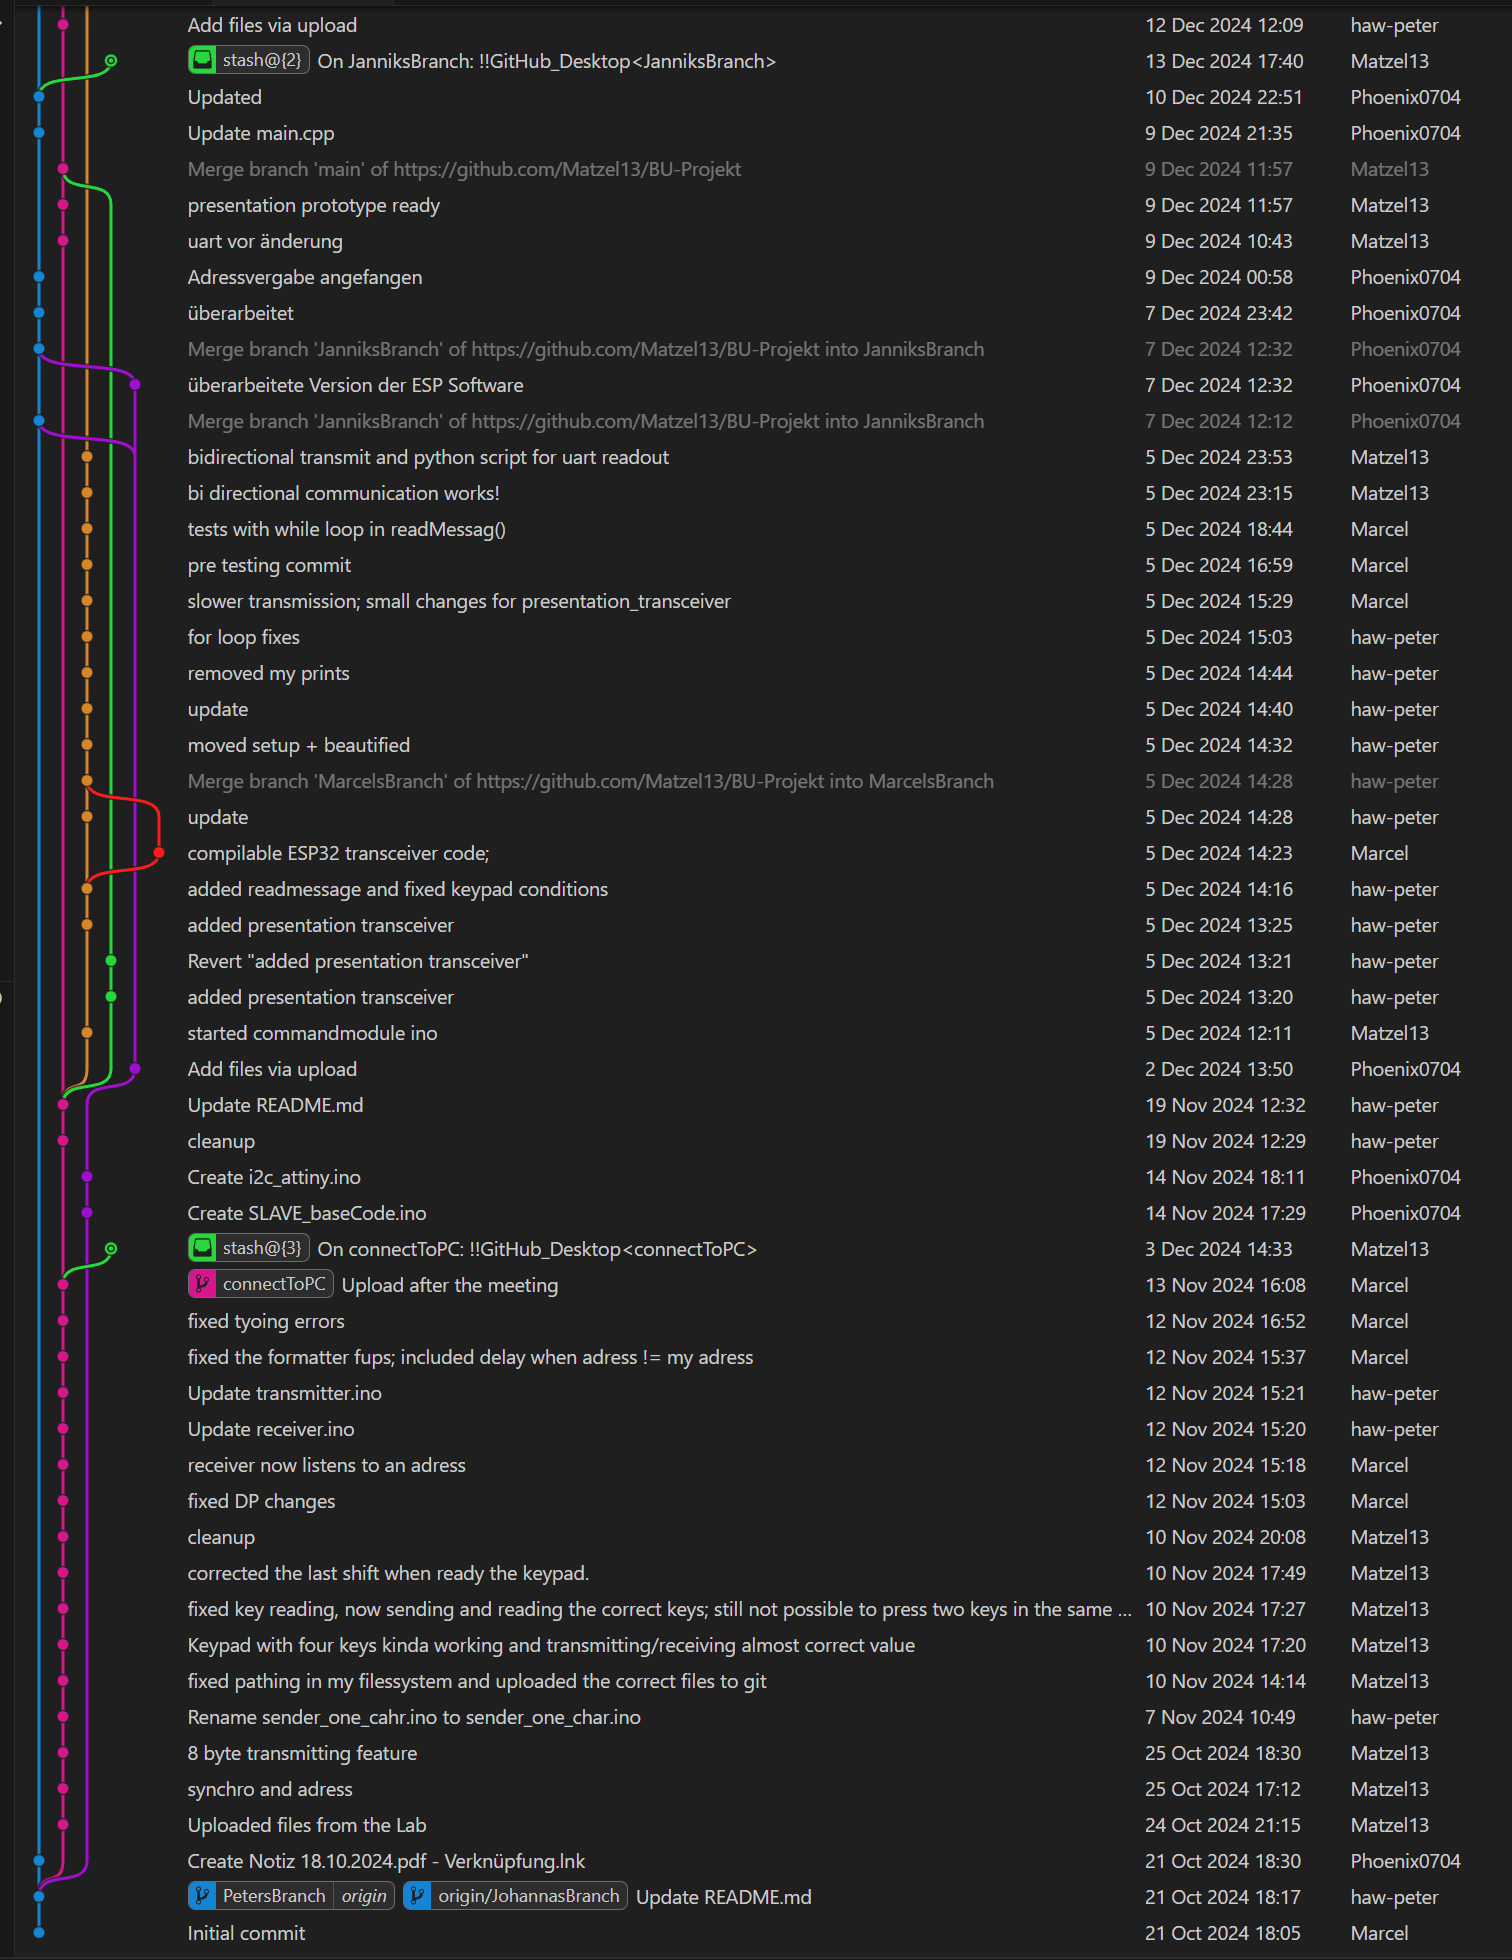
\includegraphics[width=1\textwidth]{Bilder/buGitGraph.png}}
    \caption{GitGrpah stand 12.12.2024; Commits nach dem 12.12. beziehen sich auf tex Dateien, da der Bericht auch mithilfe von Git geschrieben wurde.}
    \label{gitgraph}
\end{figure}

\subsection{Probleme}
\subsubsection{ATtiny und ATmega}
Die eingesetzten Mikrocontroller (ATtiny und ATmega) lassen sich nicht direkt über USB programmieren. Aus diesem Grund wurde innerhalb zwei Sprints der versucht, einen eigenen ISP-Programmer (In-System Programmer) zu entwickeln. Trotz vieler verfügbarer Anleitungen und Forenbeiträge zu bereits selbstgebauten Flashern gelang es nicht innerhalb des vorgegebenen Zeitrahmens, einen funktionierenden Programmer zu erstellen. Schließlich wurde ein fertiger ISP-Programmer gekauft, wodurch die Programmierung der Mikrocontroller schnell und erfolgreich möglich wurde.

\subsubsection{Differenzielle Datenübertragung}
Der erste Ansatz zum Erstellen einer differenziellen Datenübertragung war es, dies über die Software zu lösen. Jedoch kam nach gemeinsamer Absprache der Entschluss, dass dies nicht sonderlich förderlich sei und hauptsächlich der Geschwindigkeit des Busses schadet. Bei der Erweiterung des Eindraht Prototypen auf einen Zweidraht Bus mit differenzieller Datenübertragung entstand das Problem, dass in einigen Fällen die Busleitung kurzgeschlossen wird. Dieser Kurzschluss lässt sich durch galvanische Trennung der Teilnehmer vom Bus, ähnlich wie beim CAN und USB, lösen. Um weiterhin mit den zur Verfügung gestellten Produkten zu arbeiten, wurde erstmal ein Optokoppler der HAW getestet. Scheinbar war dieser Optokoppler defekt, da sich die Schaltzeiten im \si{ms} Bereich bewegt haben. Dies wäre ein viel zu hohe Latenz für die Datenübertragung und daher wurden vier mögliche alternative Bausteine bestellt, zwei verschiedene Optokoppler, einen Operationsverstärker und einen digitalen Isolator. Die Optokoppler lieferten ein zufriedenstellendes Ergebnis mit einer Latenz im einstelligen \si{\micro\second} Bereich. Zusätzlich zu den Optokopplern wurde ein Transmitter und Receiver Bauteil entdeckt, da jedoch die Lieferzeit für diese Bauteile sehr hoch ist, werden diese Bauteile vom PCB Hersteller direkt auf das PCB designt, welches das Testen der Bauteile leider nicht ermöglicht. Der aktuelle Prototyp wurde mit diskret aufgebauten Invertierern und Optokopplern realisiert.

\subsubsection{Ungetestete Bauteile}
Wie im vorherigen Absatz erwähnt, werden Bauteile benutzt, die leider im Vorfeld nicht getestet werden können. Daher wurden Alternativen im PCB-Design implementiert, falls diese Bauteile nicht die Erwartungen erfüllen. Bei der Entwicklung der PCB und der Lösung des Problems der differenziellen Datenübertragung werden die Bauteile SN65LVDT2D und SN65LVS1D benutzt. Aufgrund der erwähnten Lieferzeit konnten die Bauteile nicht getestet werden. Um etwaige Probleme mit den Bauteilen zu umgehen, werden mehrere Jumper ins Design geplant, um die Bauteile mit Optokopplern oder eine externe Testschaltung oder Testbauteil zu ersetzen.

\subsubsection{Krankheit und Lieferzeiten}
Aufgrund von Krankheiten konnte die Gruppe nicht an jedem Termin vollständig arbeiten, oder musste bereits fertige Pläne umstrukturieren. Zusätzlich kam es zu Verzögerungen durch Lieferzeiten von ein bis zwei Wochen der Bauteile.

%Bild von Zeitplan einfügen PETER EDIT: Zeitplan muss aktualisiert werden MARCEL Edit: mache ich immer schon ;) PETER EDIT: Nice, machen wir nachher rein MarcelEdit: klar ;)

Einen groben Übersichtsplan des Zeitmanagements ist in \ref{zeitplan} zu sehen. Deutlich erkennbar sind die KW44 und KW48, in denen kein Meeting stattfinden konnte. Zusätzlich sind alle Vorlesungszeiten mit im Plan aufgenommen, da die Vorlesungen teilweise genutzt wurden, um am Projekt zu arbeiten. Der Zeitplan dient lediglich einer groben Analyse der investierten Zeit und hat keinen Einfluss auf das Vorgehen.

\begin{figure}[H]
    \centering    
    \fbox{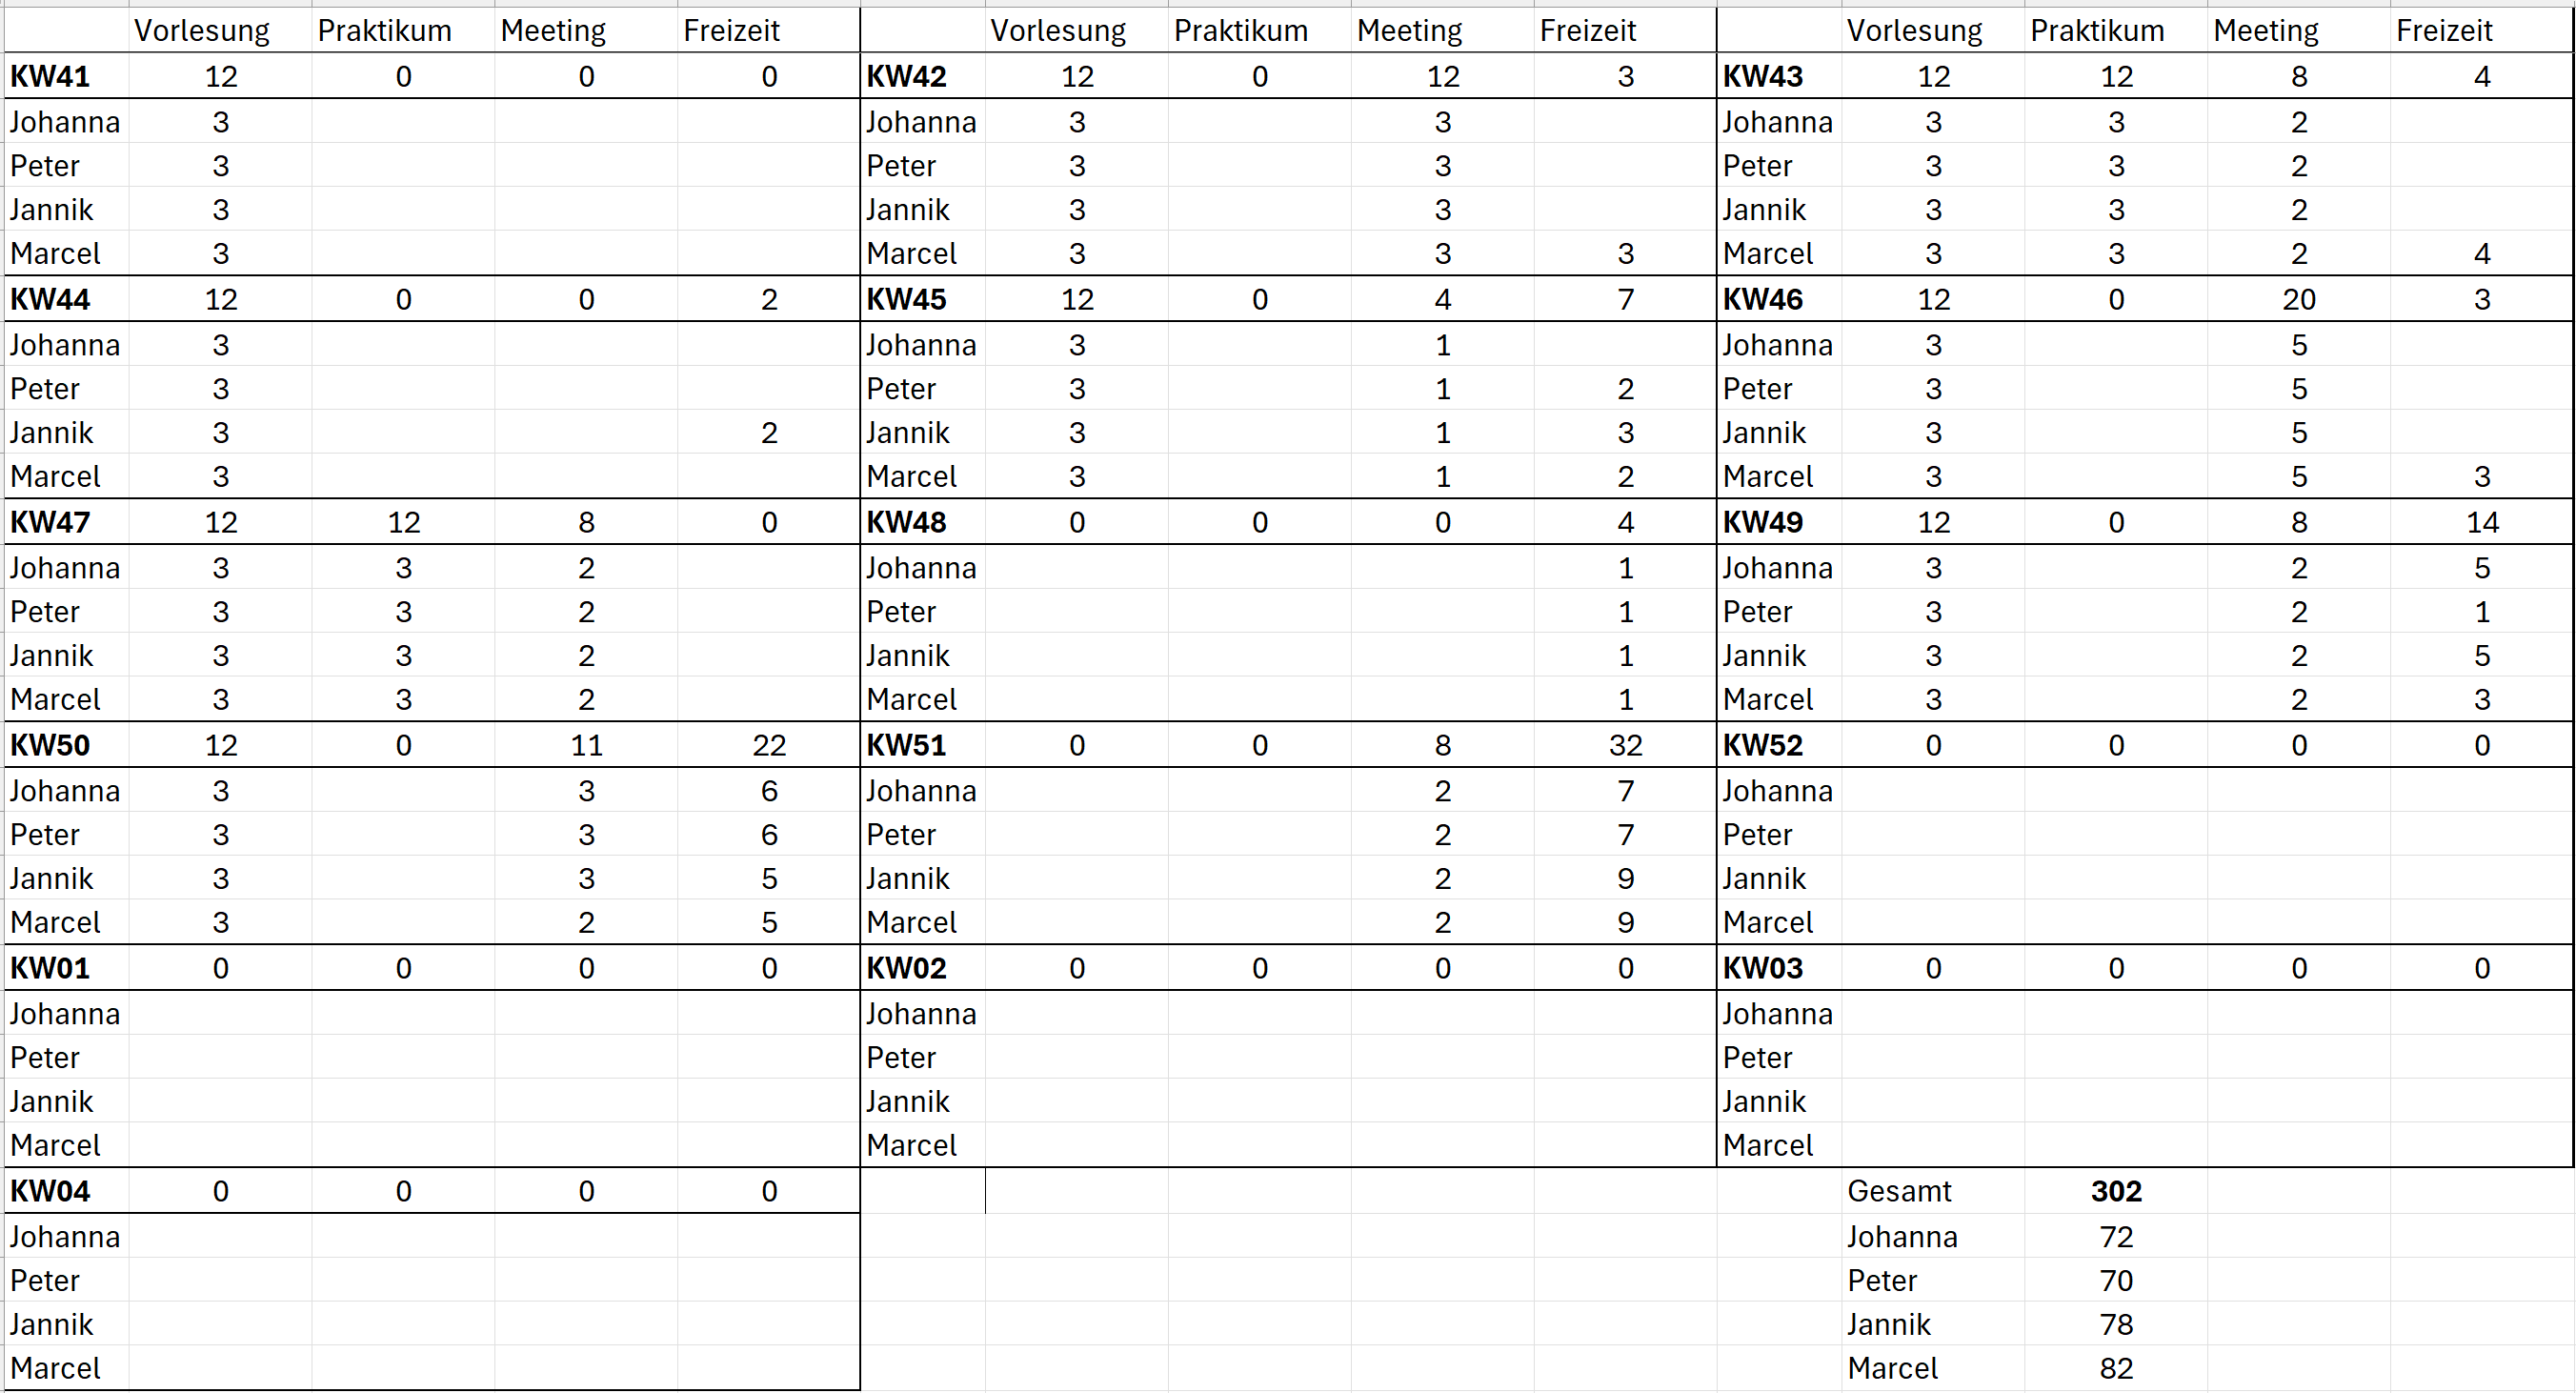
\includegraphics[width=1\textwidth]{Bilder/zeitplanBU.png}}
    \caption{Zeitmanagement stand 17.12.2024}
    \label{zeitplan}
\end{figure}


\subsection{Weiteres Vorgehen}
In den letzten Wochen der Projektzeit liegt der Fokus in der Fertigstellung eines Vorführmodells. Dazu müssen die PCBs bestellt und bestückt werden. Zusätzlich wird das grobe Gehäusedesign aus dem ersten Sprint weiterentwickelt, modelliert und mit einem 3D-Drucker gedruckt werden. \\\\
Die Software der Module wird auf einen gut leserlichen und einfach weiterzuentwickelnden Stand gebracht. Ähnlich wie bei CAN oder USB soll nach der Kommunikation zwischen zwei Teilnehmern eine Fehlererkennung laufen und eine fehlerhafte Nachricht ignoriert werden. Um Sicherzustellen, dass innerhalb der Datenübertragung keine Vier Aufeinanderfolgenden LOW-Value gesendet wollen, wird das Prinzip des Bitstuffing einsetzen.  \\\\
Eine ausgereiftere Software zum Auslesen der Daten des Hauptmoduls soll noch geschrieben werden. Diese soll dem Nutzer ermöglichen für die angeschlossenen Module verschiedene Funktionen zuzuweisen, zum Beispiel einer Taste auf einer Tastatur eine Tastenkombination zu legen. Diese Zuweisungen sollen dann in einem dict-Format gespeichert und in einer JSON Datei abgelegt, damit die Einstellungen bei Neustart des PCs noch vorhanden sind. Zusätzlich soll die Software eine Benutzeroberfläche erhalten. \\\\
Im Anschluss an die oben genannten Punkte wird mit der Entwicklung weiterer Module begonnen. Durch die verallgemeinerte Entwicklung des ersten Moduls sollte die Entwicklung weiterer Module relativ einfach sein, da sich lediglich mit der Funktion des Moduls auseinandergesetzt werden muss. Der Kommunikation zwischen dem Modul-Mikrocontrollers und dem Hauptmodul ist im Grunde die gleiche.
